\chapter{Numerical simulations}


\section{The atomic energy levels and Rydberg interaction}
We first summarize the energy levels that involved 
$\{\ket{0},\ket{1},\ket{e_F},\ket{r},\ket{r'}\}$ for two-photon process
and $\{\ket{0},\ket{1},\ket{r_m}\}$ for single-photon process.
Specifically, they correspond to the following atom states in $^{87}\mathrm{Rb}$ atoms with $I = 3/2$:
\begin{align}
&\ket 0=\ket{5S_{1/2},F=1,m_F=0},\qquad\ket1=\ket{5S_{1/2},F=2,m_F=0},\\
&\ket{e_{F}}=\ket{6P_{3/2},F,m_F=-1},\quad F=1,2,3,\\
&\ket r=\ket{70S_{1/2},m_J=-1/2}, \qquad\ket{r'}=\ket{70S_{1/2},m_J=1/2},\\
&  \ket{r_m}=\ket{53P_{3/2},m_J}, m_J = -3/2,-1/2,1/2,3/2.
\end{align}

The hyperfine state can be decomposed into the following basis:
\begin{align}
    \ket1
    &=\frac{
    \ket{m_J=\tfrac12,m_I=-\tfrac12}
    +\ket{m_J=-\tfrac12,m_I=\tfrac12}
    }{\sqrt2}
    ,\,\,\, \ket0
    =\frac{-\ket{m_J=\tfrac12,m_I=-\tfrac12}
    +\ket{m_J=-\tfrac12,m_I=\tfrac12}}{\sqrt2}.
\end{align}
The dipole interaction writes $V_{\rm dd}(\hat{R})=\frac{1}{4\pi\epsilon_0 R^{3}}[\mathbf{d}_A\cdot \mathbf{d}_B - 3(\mathbf{d}_A\cdot \hat{R})(\mathbf{d}_B\cdot \hat{R})]$.
Each vector $\mathrm{d}_A,\mathrm{d}_B$ are $j = 1$ representation of $SO(3)$ group, whose tensor product can be decomposed into the irreducible representations of $SO(3)$ group through the basis:
\begin{align}
    &[\mathbf{d}_{A}\otimes \mathbf{d}_B]_{+2}^{(2)}=\mathbf{d}_{A,+1}\mathbf{d}_{B,+1},\quad [\mathbf{d}_{A}\otimes \mathbf{d}_B]_{-2}^{(2)}=\mathbf{d}_{A,-1}\mathbf{d}_{B,-1},\\
    &[\mathbf{d}_{A}\otimes \mathbf{d}_B]_{+1}^{(2)}=\frac{1}{\sqrt{2}}(\mathbf{d}_{A,+1}\mathbf{d}_{B,0}+\mathbf{d}_{A,0}\mathbf{d}_{B,+1}),\quad [\mathbf{d}_{A}\otimes \mathbf{d}_B]_{-1}^{(2)}=\frac{1}{\sqrt{2}}(\mathbf{d}_{A,-1}\mathbf{d}_{B,0}+\mathbf{d}_{A,0}\mathbf{d}_{B,-1}),\\
    &[\mathbf{d}_{A}\otimes \mathbf{d}_B]_{0}^{(2)}=\frac{1}{\sqrt{6}}(\mathbf{d}_{A,+1}\mathbf{d}_{B,-1}+\mathbf{d}_{A,-1}\mathbf{d}_{B,+1}+2\mathbf{d}_{A,0}\mathbf{d}_{B,0}),
\end{align}
for $d_0=d_z, d_{+1} = -(d_x + i d_y)/\sqrt{2}$, and $d_{-1} = (d_x - i d_y)/\sqrt{2}$.
These basis satisfied the identity
\begin{align}
&\langle n_s l_s j_s m_s ; n_tl_t j_t m_t|[\mathbf{d}_A\otimes\mathbf{d}_B]_q^{(2)}|n ljm_A;n ljm_B\rangle=\sum_{p_A p_B}\langle n_s l_s j_s m_s|\mathbf{d}_{p_A}|n l j m_A\rangle\langle n_t l_t j_t m_t|\mathbf{d}_{p_B}|n l j m_B\rangle,\\
& 
\langle n'l'j'm'|rp|nljm \rangle=(-1)^{j+l'-1/2}C_{jm1p}^{j'm'}\sqrt{2j+1}\left\{\begin{matrix}
l & {1}/{2}   & j \\
j' & 1    & l' \\
\end{matrix}
\right\} \langle n'l' \| r \| nl\rangle.
\end{align}
In the case $\hat{R} = \hat{z}$, we noted that $V_{\mathrm{dd}}(\hat{z})$ can be represented as
\begin{align}
   V_{\mathrm{dd}}(\hat{z}) = -\frac{\sqrt{6}}{4 \pi \epsilon_0 R^3} [d_A \otimes d_B]_{0}^{(2)},
\end{align}
thus only induces the transition for $\Delta m = 0$ for state under the axis $\hat{z} = \hat{R}$. To generalized arbitrary direction, we rotated it to the arbitrary direction $\hat{R}$ by the Wigner D-matrix:
\begin{align}
    V_{\mathrm{dd}}(R,\theta, \phi)=- \frac{\sqrt{6}}{4\pi\epsilon_0 R^3} \sum_{q=-2}^{2} (-1)^q C_{-q}^{(2)}(\theta, \phi) [d_A^{(1)} \otimes d_B^{(1)}]_{q}^{(2)},
\end{align}
with the function
\begin{align}
C_{-q}^{(2)}(\theta, \phi)=\left\{\begin{aligned}
&\sqrt{\frac{3}{8}} \sin^2 \theta e^{ \mp 2i\phi}, q=\pm 2, \\
&\sqrt{\frac{3}{2}} \sin \theta \cos \theta e^{\mp i\phi}, q=\pm 1, \\
&\frac{1}{2} (3 \cos^2 \theta - 1), q = 0
\end{aligned}
\right.
\end{align}

Combining the above two results, we are able to calculate the $\langle \nu'|V_{\mathrm{dd}}(\hat{R})|\nu\rangle$ for arbitrary direction Zeeman resolved basis $\ket{\nu} = \ket{nljm}$ on direction $\hat{R}$.
Based on this, we get the Rydberg interaction matrix
\begin{align}
    H_{\mathrm pair}(R,\theta,\phi;B)=\sum_{\nu}\epsilon_{\nu}(B)|\nu\rangle\langle\nu|+V_{\mathrm{dd}}(R,\theta,\phi),
\end{align}
The driving laser $D = {\Omega}/{2}\ket{r}\bra{1} + \mathrm{h.c.}$ coupling $\ket{1r}$ to the eigenvectors $\{\ket{\Psi_k}, E_k\}$ of $H_{\mathrm pair}(R,\theta,\phi;B)$ through 
\begin{align}
    \bra{\Psi_k}D\ket{1r} = \frac{\Omega}{2}\langle \Psi_k|rr \rangle, \quad \Delta_k = E_k - E_{1r} - \hbar\omega_L.
\end{align}
Thus, it is plausible to numerically diagonalize the $V_{\mathrm{dd}}$ to get the eigenvalues $E_k$ and eigenvectors overlaps$\langle rr|{\Psi_k}\rangle$ to get the effective Hamiltonian $H_{\rm eff}$. In the following, we list these results for the case $53P_{3/2}$ and $70S_{1/2}$ states for $^{87}\mathrm{Rb}$ atoms.

\paragraph{Rydberg interaction spectra of the $53P_{3/2}$ and $70S_{1/2}$ states.}
Figure~\ref{fig:pair-spectrum-53p-70s-20g} compares the optically bright pair
spectra at $B=20\,\mathrm{G}$ for three representative orientations.  The
$53P_{3/2}$ doorway is ``unclean'' in a specific sense: its bright weight is
either left almost unshifted or divided among several orientation-dependent
pair eigenstates close to resonance.  This follows from the angular structure
of the $P$ manifold and its mixing with nearby pair channels, and rules out a
direction-independent scalar $C_6/R^6$ shift.

To make the comparison explicit, define
$c_k=\langle\Psi_k|rr\rangle$, $p_k=|c_k|^2$, and the interaction shift
$u_k=(E_k-E_{rr}^{(0)})/\hbar$.  At the representative mixed geometry
$R=3\,\mu\mathrm{m}$ and $\theta=45^\circ$, the five largest-overlap
eigenchannels are listed below.  Each entry gives
$u_k/(2\pi)$ in MHz followed by $p_k$ in brackets, and the channels are
ordered by decreasing $p_k$ rather than by energy:
\begin{align}
\begin{array}{c|ccccc}
 & |\Psi_1\rangle & |\Psi_2\rangle & |\Psi_3\rangle
 & |\Psi_4\rangle & |\Psi_5\rangle \\
\hline
53P_{3/2}
 & -5.35\,[0.472] & -66.7\,[0.276] & +25.1\,[0.207]
 & +537\,[0.028] & +97.2\,[0.010] \\
70S_{1/2}
 & +851\,[0.533] & -1731\,[0.153] & -516\,[0.113]
 & -477\,[0.102] & -427\,[0.021]
\end{array}
\label{eq:bright-pair-channels-20g}
\end{align}
Writing $P_m\equiv|53P_{3/2},m_J=m\rangle$, $|\Psi_1\rangle$ mixes
$|P_{-3/2}P_{-3/2}\rangle$ with $|P_{-1/2}P_{-1/2}\rangle$ and exchanged
$|P_{-3/2}P_{+1/2}\rangle$ components.  The states $|\Psi_2\rangle$ and
$|\Psi_3\rangle$ mix the target doorway mainly with exchanged
$|P_{-3/2}P_{-1/2}\rangle$ components; $|\Psi_4\rangle$ is predominantly the
symmetric $|53S;54S\rangle$ F\"orster channel, and $|\Psi_5\rangle$ is another
Zeeman-mixed $53P+53P$ state involving $m_J=+1/2$.  Thus the target component
is not merely accompanied by remote dark
spectators: most of it lies in three channels whose shifts are comparable to
the gate-driving scale.  In the axial geometry the same doorway instead forms
one nearly unshifted bright branch.  Consequently the eigenchannels must be
recomputed for each $(R,B,\theta)$ rather than reused with a rescaled
interaction strength.

Within a five-channel target-doorway truncation, the corresponding two-atom
Hamiltonian is
\begin{align}
H^{(5)}(t)
={}&H_{\leq 1}(t)
+\hbar\sum_{k=1}^{5}[u_k-2\Delta_L(t)]
|\Psi_k\rangle\langle\Psi_k| \nonumber\\
&+\frac{\hbar}{2}\sum_{k=1}^{5}
\left[
c_k|\Psi_k\rangle
(\Omega_A(t)\langle 1r|+\Omega_B(t)\langle r1|)+\mathrm{h.c.}
\right],
\label{eq:five-channel-pair-hamiltonian}
\end{align}
where $H_{\leq1}$ contains the ground and singly excited manifolds and the
target single-Rydberg state has rotating-frame energy $-\hbar\Delta_L(t)$.
Equivalently,
for equal in-phase drives $\Omega_A=\Omega_B=\Omega$, the symmetric state
$|W_r\rangle=(|1r\rangle+|r1\rangle)/\sqrt{2}$ couples to channel $k$ with
amplitude $\hbar\Omega(t)c_k/\sqrt{2}$.  The coupling is therefore set by the
amplitude $c_k$, not by treating $p_k$ as a Rabi frequency.  The five displayed
$53P_{3/2}$ channels capture more than $99\%$ of the target-doorway weight in
the present truncated basis at this geometry, but a high-accuracy calculation
must still verify convergence with additional channels and a larger pair
basis.  For the full $\sigma^-$ model containing a garbage Rydberg state,
$c_k$ must be replaced by the overlap matrix
$c_{k,\alpha\beta}=\langle\Psi_k|r_\alpha r_\beta\rangle$; the five channels
ranked only by $|rr\rangle$ overlap define the target--target block, not the
entire gate Hamiltonian.

The detuning from the singly excited target manifold to pair channel $k$ is
$d_k(t)=u_k-\Delta_L(t)$.  The pair sector becomes $70S$-like in the
deep-blockade limit
\begin{align}
|d_k(t)|\gg |\Omega(t)c_k|/\sqrt{2}
\qquad\text{for every optically bright channel.}
\label{eq:multichannel-blockade-condition}
\end{align}
The pair states can then be adiabatically eliminated.  Their leading effects
on $|W_r\rangle$ are summarized by two different inverse moments,
\begin{align}
\frac{\delta E_{W}}{\hbar}
&\simeq-\frac{|\Omega|^2}{2}\sum_k\frac{p_k}{d_k},
&
P_{\mathrm{pair}}
&\propto\frac{|\Omega|^2}{2}\sum_k\frac{p_k}{d_k^2}.
\label{eq:multichannel-blockade-moments}
\end{align}
For the $70S_{1/2}$ benchmark, the bright weight is also multichannel, but all
significant channels remain far from resonance in the geometries shown; this
is why it admits the deep-blockade reduction while the present $53P_{3/2}$
doorway does not.  A still stronger reduction to one literal scalar
$V|rr\rangle\langle rr|$ requires either one dominant eigenchannel or a narrow,
same-sign cluster of bright detunings, so that the two inverse moments can be
reproduced by the same $V$.  Otherwise the phase shift and blockade leakage require
separate effective parameters even for $70S$.  This reduction concerns the
pair sector only: the single-photon and two-photon single-atom Hamiltonians
remain different.

\begin{figure}[tb]
    \centering
    % Source: results/297_to_calibration/README.md; generated by scripts/check_297_pair_channels.py
    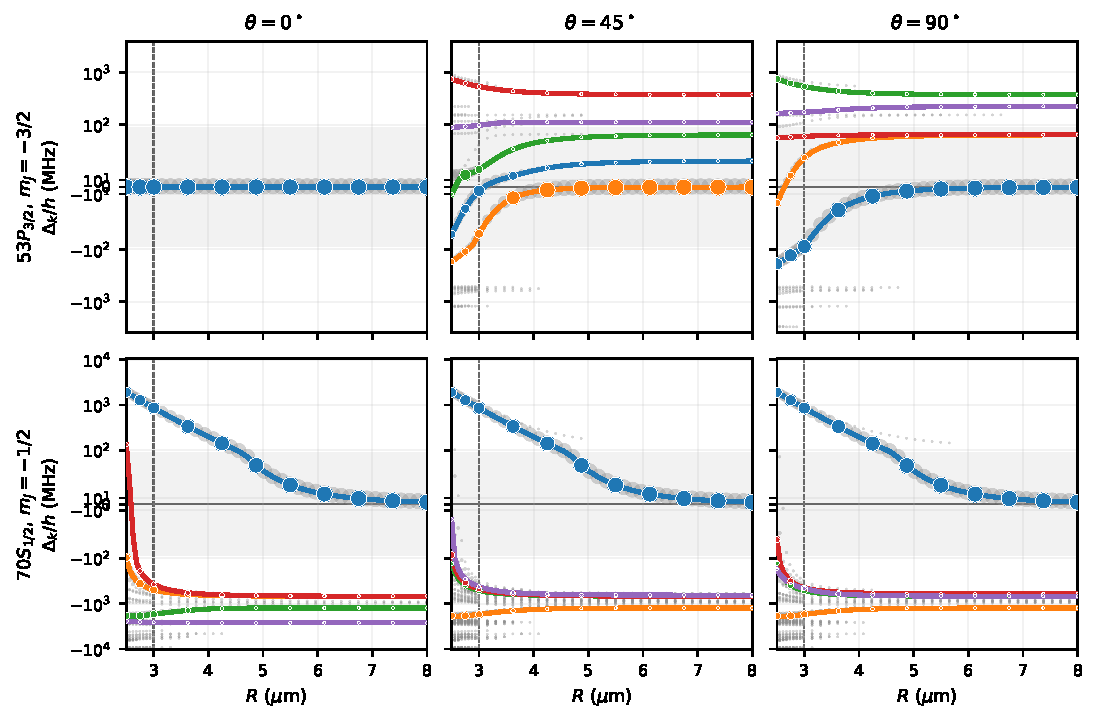
\includegraphics[width=\textwidth]{figures/pair_spectrum_53P_70S_B20G.pdf}
    \caption{Optically bright pair spectra for the $53P_{3/2},m_J=-3/2$
    doorway (top) and the $70S_{1/2},m_J=-1/2$ benchmark (bottom) at
    $B=20\,\mathrm{G}$.  Columns show three orientations of the internuclear
    axis relative to the quantization axis.  Colored curves track the five
    largest-overlap branches selected at $R=3\,\mu\mathrm{m}$, marker area is proportional to
    $p_k=|\langle rr|\Psi_k\rangle|^2$, the dashed line marks the gate spacing,
    and the shaded band denotes the weak-shift window.  The $53P_{3/2}$
    doorway retains orientation-dependent bright weight near resonance,
    whereas the $70S_{1/2}$ bright spectrum remains strongly shifted.}
    \label{fig:pair-spectrum-53p-70s-20g}
\end{figure}

\paragraph{The polarization of Rydberg lasers.}
Different polarization of Rydberg lasers couple the different Zeeman resolved basis.
Given the polarization $(\epsilon_+, \epsilon_-)$ on the wave vector $\hat{k}$ of the Rydberg laser, the polarization vector on direction $\hat{B}$ is calculated as
\begin{align}
 \epsilon_{\pm}^{(B)} = \frac{1 \pm \cos\theta}{2} \epsilon_+ + \frac{1 \mp \cos\theta}{2} \epsilon_-, \qquad \epsilon_0^{(B)} = -\frac{\sin\theta}{2} \epsilon_+ + \frac{\sin\theta}{2} \epsilon_-,
\end{align}


\subsection{The Single-photon Hamiltonian}

The $\sigma^-$, $\pi$, and $\sigma^+$ laser polarizations couple the clock
states to the Zeeman-resolved Rydberg states along the paths
\begin{align}
&\sigma^-:
\left\{
\begin{aligned}
&\ket{5S_{1/2},m_J=-1/2, m_I=1/2} \xrightarrow{} \ket{53P_{3/2},m_J=-3/2, m_I=1/2},\\
&\ket{5S_{1/2},m_J=1/2, m_I=-1/2}  \xrightarrow{\gamma} \ket{53P_{3/2},m_J=-1/2, m_I=-1/2}
\end{aligned}
\right. \\
&\sigma^+:
\left\{
\begin{aligned}
&\ket{5S_{1/2},m_J=-1/2, m_I=1/2} \xrightarrow{\gamma} \ket{53P_{3/2},m_J=1/2, m_I=1/2},\\
&\ket{5S_{1/2},m_J=1/2, m_I=-1/2} \xrightarrow{} \ket{53P_{3/2},m_J=3/2, m_I=-1/2}
\end{aligned}
\right.\\
&\pi:
\left\{
\begin{aligned}
&\ket{5S_{1/2},m_J=-1/2, m_I=1/2} \to \ket{53P_{3/2},m_J=-1/2, m_I=1/2},\\
&\ket{5S_{1/2},m_J=1/2, m_I=-1/2} \to \ket{53P_{3/2},m_J=1/2, m_I=-1/2}.
\end{aligned}
\right.
\end{align}

\subsection{The two-photon Hamiltonian}
Two-photon process use the 420-nm beam, which is assumed to be pure $\sigma_-$, and the 1013-nm beam, which is assumed to drive the target Rydberg state through the corresponding $\sigma_+$ leg.
The target Hamiltonian before choosing the optical rotating frame is:
\begin{align}
&H_P(t)
=-\varepsilon_0\ket0\bra0  + \sum_{F=1}^3 \varepsilon_F\ket{e_{F}}\bra{e_{F}} + (\varepsilon_r-\Delta_{\mathrm{add}}(t))\ket r\bra r + (\varepsilon'_r-\Delta_{\mathrm{add}}(t))\ket{r'}\bra{r'} \\
& V(t) =
\sum_{F=1}^3 \sum_{a \in \{0,1,r,r'\}}
\left[
\frac{\Omega_{Fa}(t)e^{i\Phi_{Fa}(t)}}{2}\ket{e_{F}}\bra a
+\mathrm{h.c.}\right].
\end{align}
The optical phases contain the fast rotating terms, i.e.,
\begin{align}
&\Phi_{F0}(t)=\Phi_{F1}(t) = \phi_{\mathrm{420}}(t) - \omega_{\mathrm{420}} t, \quad \Phi_{Fr}(t) = \Phi_{Fr'}(t) =\phi_{\mathrm{1013}}(t) + \omega_{\mathrm{1013}}t.
\end{align}
We first use a unitary transformation $\ket{\psi} \to U\ket{\psi}$, $H = U H U^\dagger + i (\partial_t U) U^\dagger$ to transform the inherent energy level shifts to the driving frequency. A convenient optical-frame transformation matching the convention is
\begin{align}
&U_{\rm opt}(t) =
\exp\left[
-i\sum_{F'=1}^3\theta_{e}(t)\ket{e_{F'}}\bra{e_{F'}}
-i\theta_r(t)\left(\ket r\bra r + \ket{r'}\bra{r'}\right)\right],\\
&i\partial_t U_{\rm opt}(t)U^\dagger_{\rm opt}(t) = \sum_{F'=1}^3\dot\theta_{e}(t)\ket{e_{F'}}\bra{e_{F'}} + \dot\theta_r(t)\left(\ket r\bra r + \ket{r'}\bra{r'}\right).
\end{align}
The phases are chosen so that the 1013-nm couplings are time independent,
while the 420-nm couplings carry one residual programmed phase. In particular,
for the target ladder one may choose the gauge such that
\begin{align}
\theta_{e}(t)-\theta_r(t)= \omega_{\mathrm{1013}}t,
\quad
\theta_{e}(t) =  -\omega_{\mathrm{420}} t,
\end{align}
which solve to the result $\dot\theta_{e}(t) = -\omega_{\mathrm{420}}, \quad \dot\theta_r = (-\omega_{\mathrm{1013}} -\omega_{\mathrm{420}})$.
Defining
\begin{align}
\Delta_e = \varepsilon_{F = 2}  - \omega_{\mathrm{420}}, \quad
\Delta_r = \varepsilon_r - \omega_{\mathrm{1013}} - \omega_{\mathrm{420}}, \quad 
\delta_r = \varepsilon_r' -  \varepsilon_r.
\end{align}
We choose the gauge such that $\Delta_r = 0$.
For the single-atom effective model below, we keep the three-dimensional
subspace
$P_3=\ket0\bra0+\ket1\bra1+\ket r\bra r$ and eliminate
$Q_4=\sum_{F=1}^3\ket{e_F}\bra{e_F}+\ket{r'}\bra{r'}$ in one step.
Let $\mathcal A=\{0,1,r\}$.
The Hamiltonian in this rotating frame is decomposed with respect to $P_3\oplus Q_4$ as
\begin{align}
&H_{\rm rot}(t)
=H_0(t) +V_{\rm od}(t), \quad V_{\rm od}(t)=\sum_{a\in\mathcal A}\sum_{F=1}^3g_{Fa}(t)\ket{e_F}\bra a + \mathrm{h.c.},\label{eq:7level_Vod}\\
H_0&=-\varepsilon_0\ket0\bra0
+\sum_{F=1}^3\delta_F\ket{e_F}\bra{e_F}
+ (\delta_r - \Delta_{\mathrm{add}}(t))\ket{r'}\bra{r'} \\
&\quad + \sum_{F=1}^3 \left(g_{Fr'}(t)\ket{e_F}\bra{r'}+g_{Fr'}^*(t)\ket{r'}\bra{e_F}\right) -\Delta_{\mathrm{add}}(t) \ket r\bra r, \label{eq:7level_H0}
\end{align}
where $ g_{Fa}(t)={\Omega_{Fa}(t)e^{i\phi_a(t)}}/{2}, \phi_0=\phi_1=\phi_{\mathrm{420}},\phi_r=\phi_{r'}=\phi_{\mathrm{1013}}$.
Here $\delta_F$ indicates the hyperfine shift of the $\ket{6P_{3/2},F= 1,2,3}$ state relative to the $\ket{5S_{1/2},F=2,m_F=-1}$ state with fixed value
\begin{align}
\delta_{F = 1}=\Delta_e - 2\pi\times 51\,{\rm MHz},\qquad
\delta_{F = 2}=\Delta_e,\qquad
\delta_{F = 3}=\Delta_e + 2\pi\times 87\,{\rm MHz}.
\end{align}
The $\varepsilon_0$ is the gap between the $\ket{0}$ and $\ket{1}$ states. For $^{87}\mathrm{Rb}$ atoms, $\varepsilon_0 = 2\pi \times  6.835\,{\rm GHz}$.
After specifying the realistic Hamiltonian, we eliminate $Q_4$ and retain
$P_3$.  Their ranges are
\begin{align}
\operatorname{Ran}P_3
&=\operatorname{span}\{\ket0,\ket1,\ket r\},&
\operatorname{Ran}Q_4
&=\operatorname{span}\{\ket{e_1},\ket{e_2},\ket{e_3},\ket{r'}\}.
\end{align}
Below we write $P:=P_3$ and $Q:=Q_4$.
The important point is that the $\ket{e_F}\leftrightarrow\ket{r'}$ couplings
are part of the unperturbed $Q_4$ block and are not expanded in powers of
their ratio to the bare $r$--$r'$ splitting.  Only the coupling $V_{\rm od}$
between $P_3$ and $Q_4$ is treated perturbatively, then
\begin{align}
H_P:=PH_0P&=\sum_{a\in\mathcal A}E_a\ket a\bra a,
\quad 
E_0=-\varepsilon_0,
E_1=0,
E_r=-\Delta_{\rm add}(t).
\label{eq:P3_bare_energies}
\end{align}
Set $H_Q:=QH_0Q$.  Following the sign convention in
Eq.~\eqref{eq:7level_H0}, define
$\mathbf v_a:=(g_{1a},g_{2a},g_{3a})^T,
a\in\{0,1,r,r'\}$
and introduce for $a\in\mathcal A$
\begin{align}
\Lambda_a
&:=
\operatorname{diag}\left(
\frac{1}{\delta_1-E_a},
\frac{1}{\delta_2-E_a},
\frac{1}{\delta_3-E_a}
\right),
&
\kappa_a
&:=\delta_r-\Delta_{\rm add}(t)-E_a.
\label{eq:dressed_resolvent_parameters}
\end{align}
In the ordered $Q_4$ basis
$\{\ket{e_1},\ket{e_2},\ket{e_3},\ket{r'}\}$, the shifted $Q$-block is
\begin{align}
M_a
:=H_Q-E_aQ =
\begin{pmatrix}
\Lambda_a^{-1}&\mathbf v_{r'}\\
\mathbf v_{r'}^\dagger&\kappa_a
\end{pmatrix}.
\label{eq:dressed_Q_block}
\end{align}
Assuming the indicated inverses exist, its $e_F$-sector resolvent is
\begin{align}
G_a
&:=\left[M_a^{-1}\right]_{ee}=
\Lambda_a
+
\Lambda_a\mathbf v_{r'}
\frac{1}{
\kappa_a-\mathbf v_{r'}^\dagger\Lambda_a\mathbf v_{r'}
}
\mathbf v_{r'}^\dagger\Lambda_a.
\label{eq:dressed_ee_resolvent}
\end{align}
The second term in Eq.~\eqref{eq:dressed_ee_resolvent} resums all repeated
paths through $\ket{r'}$ within $Q_4$.
In particular, no expansion in
$\|\mathbf v_{r'}\|/|\delta_r|$ is made.  The relevant Schur denominator is
\begin{align}
\zeta_a
:=
\kappa_a-\mathbf v_{r'}^\dagger\Lambda_a\mathbf v_{r'}.
\label{eq:dressed_schur_denominator}
\end{align}
Thus a small bare $r$--$r'$ splitting is treated by the full resolvent rather
than by a bare denominator expansion.  If $\zeta_a$ approaches zero and the
associated dressed state has nonzero $e_F$ weight, however, the resolvent
develops a pole and the $P_3$--$Q_4$ elimination fails.  The resonant dressed
state must then be moved into the retained subspace.

The relevant perturbative separation is the dressed block gap
\begin{align}
\Delta_{\rm dressed}(t)
:=
\operatorname{dist}\left(
\operatorname{spec}H_P(t),
\operatorname{spec}H_Q(t)
\right).
\label{eq:dressed_block_gap}
\end{align}
For uniform validity on a pulse interval $[0,T]$, we require
\begin{align}
\inf_{t\in[0,T]}\Delta_{\rm dressed}(t)&>0,&
\sup_{t\in[0,T]}
\frac{\|V_{\rm od}(t)\|}{\Delta_{\rm dressed}(t)}&\ll1.
\label{eq:dressed_uniform_condition}
\end{align}
A useful state-resolved mixing diagnostic is
\begin{align}
\sup_{t\in[0,T]}\max_{a\in\mathcal A}
\left\|(H_Q-E_aQ)^{-1}QV_{\rm od}\ket a\right\|\ll1.
\end{align}

\begin{theorem}[Direct effective 0-1-r Hamiltonian]
\label{thm:stark-elimination}
Within the instantaneous approximation, the effective Hamiltonian on $P_3$,
to second order in the block-off-diagonal coupling $V_{\rm od}$ but to all
orders in the internal $Q_4$ coupling $\mathbf v_{r'}$, is
\begin{align}
H_{\rm eff}^{(2)}
&=
\sum_{a,b\in\mathcal A}
\left[
E_a\delta_{ab}
-\frac12\mathbf v_a^\dagger
\left(G_a+G_b\right)
\mathbf v_b
\right]\ket a\bra b.
\label{eq:dressed_second_order_Heff}
\end{align}
In this block-coupling expansion, with $H_Q$ held fixed, the next static
correction is fourth order in $V_{\rm od}$.  Time-derivative corrections
associated with the instantaneous approximation are not included in
Eq.~\eqref{eq:dressed_second_order_Heff}.
\end{theorem}

\begin{proof}
Fix $t$, introduce a bookkeeping factor $\varepsilon$ multiplying
$V_{\rm od}$, and apply the symmetric second-order Feshbach reduction with
$P=P_3$, $Q=Q_4$, $H_P=PH_0P$, and $H_Q=QH_0Q$.  In the notation of
the theorem above, define
\begin{align}
\ket{\nu_a}
=QV_{\rm od}\ket a
=\sum_{F=1}^3g_{Fa}\ket{e_F},
\qquad
R_a=(H_Q-E_aQ)^{-1}.
\end{align}
Because $\ket{\nu_a}$ has support only on the $e_F$ sector and
$G_c=[(H_Q-E_cQ)^{-1}]_{ee}$ for $c\in\mathcal A$,
\begin{align}
\bra{\nu_a}R_c\ket{\nu_b}
=\mathbf v_a^\dagger G_c\mathbf v_b.
\end{align}
Substitution into the symmetric second-order expression gives
Eq.~\eqref{eq:dressed_second_order_Heff} after setting $\varepsilon=1$.
Since the complete
$\ket{e_F}\leftrightarrow\ket{r'}$ coupling belongs to $H_Q$, it is retained
to all orders in the resolvents $G_c$.  The dressed-gap and norm conditions
stated above ensure the hypotheses of the proposition; the state-resolved
quantity provides an additional mixing diagnostic.
\end{proof}

\begin{lemma}[Proportion of branch]
    \label{lemma:proportion-of-Omega}
   Define $\mathbf v_a=(g_{1a},g_{2a},g_{3a})^T, a\in\{0,1,r,r'\}$, then
   \begin{align}
\mathbf v_0
&=\frac{\Omega_{420}e^{i\phi_{\mathrm{420}}}}{2}
\left(\sqrt{\frac{3}{10}}+\sqrt{\frac{2}{15}},\,
-\sqrt{\frac12},\,0\right)^T, \quad
\mathbf v_1
=\frac{\Omega_{420}e^{i\phi_{\mathrm{420}}}}{2}
\left(\sqrt{\frac{3}{10}}-\sqrt{\frac{2}{15}},\,
-\sqrt{\frac12},\,\sqrt{\frac45}\right)^T,\\
\mathbf v_r
&=\frac{\Omega_{1013}e^{i\phi_{\mathrm{1013}}}}{2}
\left(\sqrt{\frac{3}{10}},\,-\sqrt{\frac12},\,\sqrt{\frac15}\right)^T, \quad
\mathbf v_{r'}
=\frac{\Omega_{1013}e^{i\phi_{\mathrm{1013}}}}{2}
\left(-\sqrt{\frac{2}{15}},\,0,\,\sqrt{\frac15}\right)^T.
\end{align}
\end{lemma}
\begin{proof}
    The 420-nm coupling is evaluated in the uncoupled $\ket{m_J,m_I}$ basis, where the electric dipole operator preserves $m_I$ and changes $m_J$ by $q=-1$. With $I=3/2$ and CG phases,
    only two components of each $\ket{e_{F'}}=\ket{6P_{3/2},F',m_F=-1}$ are reached from $m_F=0$ by $\sigma_-$:
    \begin{align}
    \begin{array}{c|cc}
    F'&
    \ket{m_J=-\tfrac32,m_I=\tfrac12}&
    \ket{m_J=-\tfrac12,m_I=-\tfrac12}\\
    \hline
    1&\sqrt{\frac{3}{10}}&-\sqrt{\frac{2}{5}}\\
    2&-\sqrt{\frac{1}{2}}&0\\
    3&\sqrt{\frac{1}{5}}&\sqrt{\frac{3}{5}}
    \end{array}
    \end{align}
    The overall phase of each $\ket{e_{F'}}$ is conventional; the phase choice above matches the signs used for the effective Rabi sum.
    Define
    \begin{align}
    \Omega_{420}(t)
    &:=
    \frac{
    \langle 6P_{3/2},m_J=-\tfrac32,m_I=\tfrac12|
    e\mathbf r\cdot\mathbf E^{(1)}_-(t)
    |5S_{1/2},m_J=-\tfrac12,m_I=\tfrac12\rangle
    }{\sqrt2\,\hbar},\\
    \gamma\,\Omega_{420}(t)
    &:=
    \frac{
    \langle 6P_{3/2},m_J=-\tfrac12,m_I=-\tfrac12|
    e\mathbf r\cdot\mathbf E^{(1)}_-(t)
    |5S_{1/2},m_J=\tfrac12,m_I=-\tfrac12\rangle
    }{\sqrt2\,\hbar}.
    \end{align}
    With the same CG phase convention, the Wigner-Eckart theorem gives
    \begin{align}
    \gamma
    =
    \frac{
    \langle 6P_{3/2},m_J'=-\tfrac12,m_I'=-\tfrac12|d_{-1}|5S_{1/2},m_J=\tfrac12,m_I=-\tfrac12\rangle
    }{
    \langle 6P_{3/2},m_J'=-\tfrac32,m_I'=\tfrac12|d_{-1}|5S_{1/2},m_J=-\tfrac12,m_I=\tfrac12\rangle
    }
    =\sqrt{{1}/{3}},
    \end{align}
    assuming ideal $\sigma_-$ polarization and no magnetic-field mixing.
    The resulting 420-nm Rabi amplitudes are
    \begin{align}
        \left\{
    \begin{aligned}
    \Omega_{F=1,1}
    &=\left(
    \sqrt{\frac{3}{10}}
    -\sqrt{\frac{2}{5}}\gamma\right)\Omega_{420}
    =  \left(
        \sqrt{\frac{3}{10}}
        -\sqrt{\frac{2}{15}}
        \right)\Omega_{420},\\
    \Omega_{F=1,0}&=\left(
    \sqrt{\frac{3}{10}}
    +\sqrt{\frac{2}{5}}\gamma
    \right)\Omega_{420}
    = \left(
        \sqrt{\frac{3}{10}}
        +\sqrt{\frac{2}{15}}
        \right)\Omega_{420},
    \end{aligned}
    \right.
    \\
    \left\{
    \begin{aligned}
    \Omega_{F=2,1}
    &=
    -\sqrt{\frac{1}{2}}\Omega_{420},\\
    \Omega_{F=2,0}
    &=
    -\sqrt{\frac{1}{2}}\Omega_{420},
    \end{aligned}
    \right.
    \qquad
    \left\{
    \begin{aligned}
    \Omega_{F=3,1}&=
    \left(
    \sqrt{\frac{1}{5}}
    +\sqrt{\frac{3}{5}}\gamma
    \right)\Omega_{420} =
        \sqrt{\frac{4}{5}}\Omega_{420},\\
    \Omega_{F=3,0}
    &=
    \left(
    \sqrt{\frac{1}{5}}
    -\sqrt{\frac{3}{5}}\gamma
    \right)\Omega_{420} =0,
    \end{aligned}
    \right.
    \end{align}
    
    For the 1013-nm leg, define
    \begin{align}
    \Omega_{1013}(t)
    &:=
    \frac{
    \langle 70S_{1/2},m_J=-\tfrac12,m_I=\tfrac12|
    e\mathbf r\cdot\mathbf E^{(2)}_+(t)
    |6P_{3/2},m_J=-\tfrac32,m_I=\tfrac12\rangle
    }{\hbar},\\
    \xi\,\Omega_{1013}(t)
    &:=
    \frac{
    \langle 70S_{1/2},m_J=\tfrac12,m_I=-\tfrac12|
    e\mathbf r\cdot\mathbf E^{(2)}_+(t)
    |6P_{3/2},m_J=-\tfrac12,m_I=-\tfrac12\rangle
    }{\hbar}.
    \end{align}
    By the Wigner-Eckart theorem,
    \begin{align}
    \xi
    &=
    \frac{
    \langle 70S_{1/2},m_J=\tfrac12,m_I=-\tfrac12|d_{+1}|6P_{3/2},m_J=-\tfrac12,m_I=-\tfrac12\rangle
    }{
    \langle 70S_{1/2},m_J=-\tfrac12,m_I=\tfrac12|d_{+1}|6P_{3/2},m_J=-\tfrac32,m_I=\tfrac12\rangle
    }
    =\sqrt{{1}/{3}},
    \end{align}
    assuming ideal $\sigma_+$ polarization and no magnetic-field mixing.
    Therefore, the target Rydberg state $\ket r=\ket{70S_{1/2},m_J=-1/2}$ is connected from the $\ket{m_J=-3/2,m_I=1/2}$ component of each $\ket{e_{F'}}$, while the off-resonant partner $\ket{r'}=\ket{70S_{1/2},m_J=1/2}$ is reached from the $\ket{m_J=-1/2,m_I=-1/2}$ component. The resulting 1013-nm Rabi amplitudes are
    \begin{align}
    &\Omega_{F = 1, r}=\sqrt{\frac{3}{10}}\Omega_{1013}, \quad
    \Omega_{F = 2, r}=-\sqrt{\frac{1}{2}}\Omega_{1013}, \quad
    \Omega_{F = 3, r}=\sqrt{\frac{1}{5}}\Omega_{1013},\\
    &\Omega_{F = 1, r'}=-\sqrt{\frac{2}{5}}\xi\Omega_{1013}=-\sqrt{\frac{2}{15}}\Omega_{1013}, \quad
    \Omega_{F = 2, r'}=0, \quad
    \Omega_{F = 3, r'}=\sqrt{\frac{3}{5}}\xi\Omega_{1013}=\sqrt{\frac{1}{5}}\Omega_{1013}.
    \end{align}
\end{proof}

\section{Pulse optimization}

We focus on the Time-dependent Hamiltonian with the form $H(\mathbf{u})=H_0+\sum_\alpha u_{\alpha}(t)H_\alpha$,
where $\mathbf{u}(t) := [u_{\alpha}(t)]_{\alpha \in \mathcal{A}}$ are different control channels.
The continues time might be sampled on $N$ time
intervals ${u}_{\alpha, k} := u_{\alpha}(t_k)$ for $k=0,\ldots,N-1$. 
Given these $k$ intervals, the parameters $u_{\alpha,k}$ are optimized by the problem
\begin{figure}[htbp!]
    \centering
    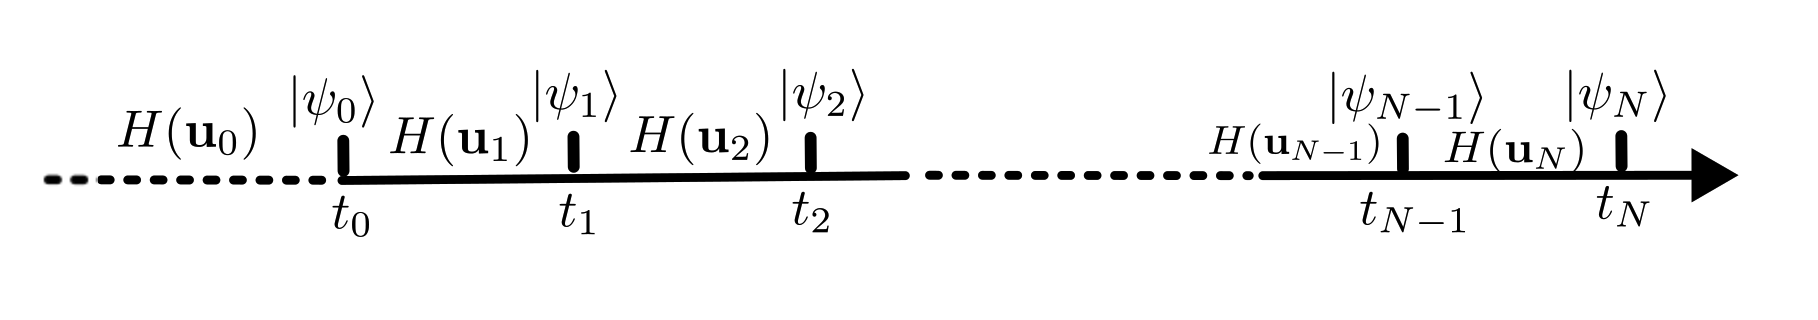
\includegraphics[width = 0.8\textwidth]{figures/GRAPE.png}
\end{figure}
\begin{align}
    &\min_{\mathbf{u}_k, U_k}J(\mathbf{u}_k,U_k)=\Phi(U_{N}, U_{\mathrm{targ}}) \qquad \text{s.t.~}U_k=\exp\left(-iH(\mathbf u_k) \Delta t_k\right)U_{k - 1}, \quad U_0 = \mathbb{I}.
\label{eq:grape_forward}
\end{align}

\subsection{GRAPE}
The Gradient-ascent pulse engineering (GRAPE)  plugs the restrictions into the target loss function, make $J(\mathbf{u}_k)=\Phi(U_{N}, U_{\mathrm{targ}})$ as a function of pulse segments $\mathbf{u}_1,\cdots,\mathbf{u}_N$ only.
Then applying the chain rule backward through this discretized evolution,
it evaluates the complete gradient $\partial J/\partial u_{\alpha,k}$.
Denoting $V_k := \exp\left(-iH(\mathbf u_k) \Delta t_k\right)$ and multiple input state $\ket{s}$ for $s\in\mathcal S$, we get 
\begin{align}\label{eq:forward}
    \ket{\psi_0^{(s)}}=\ket{s},\quad \ket{\psi_{k+1}^{(s)}}=V_k\ket{\psi_k^{(s)}}.
\end{align}
The loss function then can be first regarded as a real joint function $\Phi(\cdot)$ on properties of the final states and a restriction punishment on the control parameters $R(\cdot)$
through $J=\Phi\!\left(\left\{\ket{\psi_N^{(s)}}\right\}_{s\in\mathcal S}\right) + R(\mathbf{u})$.
A small change $u_{\alpha, k} \to u_{\alpha, k}+\delta u_{\alpha, k}$ gives the chains rule of $\psi_{k+1}^{(s)}$ through
\begin{align}
 \ket{\delta\psi_{k+1}^{(s)}}
= \delta \left[V_k \ket{\psi_{k}^{(s)}}\right]
= V_k\ket{\delta\psi_k^{(s)}}
+ \sum_\alpha \frac{\partial V_k}{\partial u_{\alpha,k}} \ket{\psi_k^{(s)}}\, \delta u_{\alpha k}.
\end{align}
We set up the dual state vector $\ket{\lambda_k^{(s)}}$ through the relation
\begin{align}\label{eq:backward}
    \ket{\lambda_N^{(s)}}=\partial \Phi /\partial \bra{\psi_N^{(s)}}, \quad 
\ket{\lambda_k^{(s)}}=V_k^\dagger\ket{\lambda_{k+1}^{(s)}}.
\end{align}
Use the identity $\delta\Phi= 2\operatorname{Re} \sum_{s\in\mathcal S} \left\langle \lambda_N^{(s)} \middle|\delta\psi_N^{(s)}\right\rangle$ and conclude:
\begin{align}
    2\mathrm{Re}\left\langle\lambda_{k+1}^{(s)}\middle|\delta\psi_{k+1}^{(s)}\right\rangle
&=2\mathrm{Re}\left\langle\lambda_{k+1}^{(s)}\middle|V_k\delta\psi_k^{(s)}\right\rangle+
2\mathrm{Re}\sum_\alpha\left\langle\lambda_{k+1}^{(s)}\middle|\frac{\partial V_k}{\partial u_{\alpha,k}}\middle|\psi_k^{(s)}\right\rangle\delta u_{\alpha,k}\\
&=2\mathrm{Re}\left\langle\lambda_{k}^{(s)}\middle|\delta\psi_k^{(s)}\right\rangle+
2\mathrm{Re}\sum_\alpha\left\langle\lambda_{k+1}^{(s)}\middle|\frac{\partial V_k}{\partial u_{\alpha,k}}\middle|\psi_k^{(s)}\right\rangle\delta u_{\alpha,k},
\end{align}
This then gives the equation
\begin{align}
\delta\Phi&=
    2\operatorname{Re}\sum_s\left\langle\lambda_0^{(s)}\middle|\delta\psi_0^{(s)}\right\rangle+\sum_{k,\alpha}2\operatorname{Re}\sum_s\left[\left\langle\lambda_{k+1}^{(s)}\middle|\frac{\partial V_k}{\partial u_{\alpha, k}}\middle|\psi_k^{(s)}\right\rangle\right]\delta u_{\alpha,k}.
\end{align}
Use the fact $\psi_0^{(s)}$ is fixed, we conclude the gradients as a vector inner products:
\begin{align}\label{eq:fb_deri}
    \frac{\partial \Phi}{\partial u_{\alpha,k}} = 2\operatorname{Re}\sum_s\left[\left\langle\lambda_{k+1}^{(s)}\middle|\frac{\partial V_k}{\partial u_{\alpha, k}}\middle|\psi_k^{(s)}\right\rangle\right].
\end{align}
Based on Eq.\eqref{eq:fb_deri}, the gradients now can be calculated through calculating the forwards and backwards propagation based on Eq.\eqref{eq:forward} and Eq.\eqref{eq:backward}, getting $\ket{\psi_k^{(s)}}$ and $\ket{\lambda_k^{(s)}}$, respectively. 
The derivative of $V_k$ can be calculated through Lemma~\ref{lem:exp_deri} as
\begin{align}
\frac{\partial}{\partial u_{\alpha, k}}  e^{-i(H_0+\sum_\alpha u_{\alpha,k}H_\alpha) \Delta t_k}&= \int_{r = 0}^1 dr e^{(1-r)S} \dot{S} e^{rS},\quad S = (-i\Delta t_k) \cdot \left[H_0 + \sum_{\alpha} u_{\alpha,k} H_{\alpha}\right].
\end{align}

\section{Scalability of a three-atom optimized ZXZ pulse}
\label{sec:zxz-scalability}

We now ask a question that is logically separate from finding a good optimum:
does a pulse optimized on three atoms implement the intended dynamics on a
longer chain?  Direct quantum optimal control is very effective at enforcing
hardware constraints on the training system, but the optimization algorithm
alone supplies no relation between different system sizes.  The distinction is
important for the ZXZ experiment of Ref.~\cite{hu2025universal}.  Its control
pulse is obtained from a three-atom unitary objective and is then reused on a
longer chain.  The arXiv v1 source and the current v5 source describe an
eight-atom experiment; v5 additionally reports a 50-atom tensor-network check
of selected local observables.  The analysis below applies without change to a
seven-atom deployment or any other chain length.  Neither the longer-chain
experiment nor the 50-atom local-observable calculation is, by itself, a
uniform channel-error bound.

For a chain of $N$ atoms with spacing $a$, write the analog Rydberg Hamiltonian
as
\begin{align}
\frac{H_N^{\mathrm{ryd}}[u;t]}{\hbar}
={}&\frac{\Omega(t)}{2}\sum_{j=1}^{N}X_j
-\Delta(t)\sum_{j=1}^{N}n_j
+\sum_{1\leq i<j\leq N}V_{|i-j|}n_i n_j,
&
V_r=\frac{C_6}{(ra)^6},
\label{eq:rydberg-zxz-family}
\end{align}
where $n_j=(I-Z_j)/2$ and $u=(\Omega,\Delta)$.  The implemented and target
unitaries are
\begin{align}
U_N[u]
&=\mathcal T\exp\left[-\frac{i}{\hbar}\int_0^T
H_N^{\mathrm{ryd}}[u;t]dt\right],
&
T_N(\vartheta)
&=\exp[-i\vartheta H_{\mathrm{ZXZ}}^{(N)}],
\label{eq:implemented-and-target-zxz}\\
H_{\mathrm{ZXZ}}^{(N)}
&=\sum_{j=2}^{N-1}K_j,
&
K_j&=Z_{j-1}X_jZ_{j+1}.
\label{eq:open-zxz-generator}
\end{align}
For definiteness, write its phase-insensitive unitary objective in the process
fidelity convention
\begin{align}
F_3[u]=\frac{1}{4^3}\left|\operatorname{Tr}
\left[T_3(\vartheta)^\dagger U_3[u]\right]\right|^2,
\label{eq:three-atom-process-fidelity}
\end{align}
with $H_{\mathrm{ZXZ}}^{(3)}=Z_1X_2Z_3$.  A large value of
$F_3$ is a statement about one eight-dimensional Hilbert space.  It does not
yet constrain the additional interaction contexts present for $N>3$.  Other
standard unitary-fidelity conventions differ numerically but do not change
this logical conclusion.

\subsection{The target is shallow, but its bulk light cone is not three sites}

The target has considerably more structure than a generic many-body unitary.
This structure makes a local-inversion analysis possible and also exposes why
three atoms are insufficient.

\begin{proposition}[Exact shallow representation of the ZXZ target]
\label{prop:zxz-shallow-representation}
All operators $K_j$ in Eq.~\eqref{eq:open-zxz-generator} commute.  If
\begin{align}
C_N=\prod_{j=1}^{N-1}\operatorname{CZ}_{j,j+1},
\end{align}
then
\begin{align}
T_N(\vartheta)
=C_N\left(\prod_{j=2}^{N-1}e^{-i\vartheta X_j}\right)C_N.
\label{eq:zxz-exact-circuit}
\end{align}
Consequently, $T_N$ has a nearest-neighbor circuit of depth five, independent
of $N$: two edge-color layers for the first $C_N$, one layer of bulk
$X$ rotations, and two layers for the second $C_N$.
\end{proposition}

\begin{proof}
Two distinct $K_j$ either have disjoint support, share only equal $Z$
operators, or have two sites on which an $X$ and a $Z$ anticommute.  The last
case produces two minus signs, so $[K_j,K_k]=0$ for all $j,k$.  A controlled-Z
gate conjugates $X_j$ to $X_jZ_k$ on an adjacent site $k$.  Hence
$C_NX_jC_N=Z_{j-1}X_jZ_{j+1}$ for every bulk site.  Since $C_N^2=I$,
functional calculus gives Eq.~\eqref{eq:zxz-exact-circuit}.
\end{proof}

Equation~\eqref{eq:zxz-exact-circuit} proves that the target itself obeys the
shallow-circuit promise in the learning theorem of Huang et
al.~\cite{huang_2024_learning}.  It does not make the analog evolution $U_N$,
or the mismatch $T_N^\dagger U_N$, an exactly shallow circuit.  Below we use
their strong local-identity lemma, which does not require shallowness, and use
a Lieb--Robinson window in place of exact shallowness for the physical
evolution.  The exact circuit does not reduce the relevant bulk neighborhood
to three atoms.  Let $c=\cos(2\vartheta)$ and
$s=\sin(2\vartheta)$.  For $3\leq i\leq N-2$, conjugation by the commuting
$K_j$ gives
\begin{align}
T_N^\dagger Z_iT_N
={}&cZ_i+sZ_{i-1}Y_iZ_{i+1},
\label{eq:zxz-heisenberg-z}\\
T_N^\dagger X_iT_N
={}&c^2X_i-cs\left(
Z_{i-2}X_{i-1}Y_i+Y_iX_{i+1}Z_{i+2}\right)\nonumber\\
&\hspace{1.3em}-s^2Z_{i-2}X_{i-1}X_iX_{i+1}Z_{i+2}.
\label{eq:zxz-heisenberg-x}
\end{align}
Indeed, for $K^2=I$,
\begin{align}
e^{i\vartheta K}Pe^{-i\vartheta K}
=
\begin{cases}
P,&[K,P]=0,\\
cP+isKP,&\{K,P\}=0.
\end{cases}
\label{eq:pauli-conjugation-rule}
\end{align}
Only $K_i$ anticommutes with $Z_i$, which gives
Eq.~\eqref{eq:zxz-heisenberg-z}.  Only the mutually commuting
$K_{i-1}$ and $K_{i+1}$ anticommute with $X_i$; applying
Eq.~\eqref{eq:pauli-conjugation-rule} twice gives
Eq.~\eqref{eq:zxz-heisenberg-x}, including the five-site term.
The image of $Y_i=iX_iZ_i$ has the same five-site support bound.  Thus the
exact backward light cone of a generic single-site Pauli in the bulk is
$\{i-2,\ldots,i+2\}$.  Three atoms contain the light cone of $Z_i$ but not
that of $X_i$ or $Y_i$ at a generic angle ($s\neq0$).  Five atoms are the
minimum target-only bulk window, before adding any buffer for propagation
under the physical Rydberg Hamiltonian.  This is our first main structural
result.

\subsection{What direct trajectory optimization proves}

The direct method in Ref.~\cite{hu2025universal} promotes every intermediate
unitary and the controls to optimization variables.  In a simplified notation
its full-unitary transcription is
\begin{align}
\min_{\{U_k,u_k,\dot u_k,\ddot u_k\}}
&\quad 1-F(U_K,T_N)+R(u)
\nonumber\\
\text{subject to}
&\quad U_{k+1}=\exp[-iH_N(u_k)\Delta t_k]U_k,
\quad U_0=I,
\label{eq:direct-qoc-transcription}\\
&\quad u_{k+1}=u_k+\dot u_k\Delta t_k,
\qquad
\dot u_{k+1}=\dot u_k+\ddot u_k\Delta t_k,
\nonumber\\
&\quad u_k,\dot u_k,\ddot u_k\ \text{satisfy the hardware bounds}.
\nonumber
\end{align}
Its principal benefit is feasibility: amplitude, slew-rate, smoothness,
duration, and robustness constraints can be imposed directly rather than
encoded only through soft penalties.  Its variables nevertheless contain a
$2^N\times2^N$ unitary at every knot.  A naive full-unitary formulation
therefore has $O(K4^N)$ stored state variables, and its sparse KKT blocks still
grow exponentially with $N$.  More importantly, solving
Eq.~\eqref{eq:direct-qoc-transcription} for $N=3$ proves only feasibility and
optimality properties of that $N=3$ nonlinear program.  Direct transcription
changes the route to an optimum; it does not create a small-to-large theorem.

\subsection{A no-go theorem for inference from the three-site fidelity}

The missing implication is not merely a weakness of a particular optimizer.
It is impossible without an additional locality promise and additional local
data.

\begin{proposition}[Three-site non-identifiability]
\label{prop:three-site-no-go}
Suppose a function $f:[0,1]\to[0,1]$ upper-bounds the normalized $N$-site
channel error by $f$ of the three-site error for every
translation-invariant family with bounded finite-range local terms.  Then
$f(0)=1$.  Hence no nontrivial bound with $f(0)<1$---in particular, no
consistent bound with $f(0)=0$---can follow from the three-site error alone:
exact agreement at $N=3$ is compatible with maximal channel error at $N=4$.
\end{proposition}

\begin{proof}
For $N\geq1$, define
\begin{align}
Q_N=\sum_{j=1}^{N-3}Z_jZ_{j+1}Z_{j+2}Z_{j+3},
\end{align}
where the empty sum is zero.  Compare the two local circuit families
\begin{align}
U_N^{(0)}=T_N,
\qquad
U_N^{(1)}=T_N\exp[-i\phi Q_N].
\end{align}
They are identical for every $N\leq3$.  For $N=4$ and $\phi=\pi/2$, their
relative unitary is $-iZ_1Z_2Z_3Z_4$.  Take an equal superposition of a
$+1$ and a $-1$ eigenvector of $Z_1Z_2Z_3Z_4$.  The identity channel and the
relative channel send this state to orthogonal states.  Their diamond distance
is therefore maximal.  Composition with the common target channel does not
change that distance.  Any proposed bound must therefore obey $1\leq f(0)$;
since its codomain is $[0,1]$, $f(0)=1$.
\end{proof}

The four-body term in this proof is a minimal information-theoretic
counterexample.  The same mechanism occurs naturally in pulse engineering.
The Magnus generator of Eq.~\eqref{eq:rydberg-zxz-family} contains nested
commutators of the form
\begin{align}
\Omega_q(T)\sim
\int dt_1\cdots dt_q
[h_{X_1}(t_1),[h_{X_2}(t_2),\ldots,h_{X_q}(t_q)]\cdots].
\label{eq:magnus-connected-clusters}
\end{align}
A nested commutator vanishes if a newly added support is disjoint from the
support accumulated before it.  Every nonzero summand therefore corresponds
to a connected cluster.  Optimizing three atoms can constrain connected
clusters of size at most three, but it is blind to all connected coefficients
whose minimum support has four or more sites.  The physical chain also
contains pair couplings at distances and in overlapping environments that do
not occur in the isolated three-atom objective.  These terms need not be
large individually; a nonzero density of them can produce an extensive error.

\subsection{Local inversions turn locality into a certificate}

We now state precisely what Ref.~\cite{huang_2024_learning} contributes.  Use
the normalized diamond distance
\begin{align}
d_\diamond(\mathcal A,\mathcal B)
=\frac{1}{2}\|\mathcal A-\mathcal B\|_\diamond
\end{align}
and define the input-side mismatch
\begin{align}
W_N[u]=T_N^\dagger U_N[u],
\qquad
\mathcal W_N=\mathcal T_N^{-1}\circ\mathcal U_N.
\label{eq:zxz-mismatch-unitary}
\end{align}
For every site, introduce the strong local residual
\begin{align}
\eta_i^{(N)}[u]
=\frac{1}{2}\sum_{P\in\{X,Y,Z\}}
\left\|W_N[u]^\dagger P_iW_N[u]-P_i\right\|_\infty.
\label{eq:strong-local-residual}
\end{align}
This is a worst-case local quantity, not a state-specific expectation value.

\begin{proposition}[Local-to-global channel certificate]
\label{prop:local-to-global-zxz}
For every $N$ and every pulse $u$,
\begin{align}
d_\diamond(\mathcal U_N[u],\mathcal T_N)
\leq
\min\left\{1,\frac{3}{2}\sum_{i=1}^{N}\eta_i^{(N)}[u]\right\}.
\label{eq:local-to-global-diamond-bound}
\end{align}
\end{proposition}

\begin{proof}
The Pauli condition in Eq.~\eqref{eq:strong-local-residual} implies that
$\mathcal W_N$ is a strong $\eta_i^{(N)}$-approximate local identity on site
$i$.  The global-identity lemma of Ref.~\cite{huang_2024_learning} gives
$\|\mathcal W_N-\mathcal I\|_\diamond\leq
3\sum_i\eta_i^{(N)}$.  Divide by two and use invariance of diamond distance
under composition with $\mathcal T_N$.
\end{proof}

This bound immediately displays the global scaling requirement.  If all bulk
residuals are bounded by one fixed number $\eta$, the certified global error is
$O(N\eta)$.  To guarantee a fixed global channel error $\epsilon$ at size
$N$, a sufficient requirement is $\eta=O(\epsilon/N)$.  A fixed nonzero local
error density cannot provide a size-independent global process fidelity.

The conclusion is different for a fixed local observable.  Expand an
observable supported on $A$ in Pauli strings,
\begin{align}
\widetilde O_A:=T_N^\dagger O_AT_N
=\sum_{\boldsymbol p}c_{\boldsymbol p}P_{\boldsymbol p},
\qquad
\|\widetilde O_A\|_{P,1}:=\sum_{\boldsymbol p}|c_{\boldsymbol p}|.
\end{align}
By Eqs.~\eqref{eq:zxz-heisenberg-z}--\eqref{eq:zxz-heisenberg-x}, its support
is contained in the two-site enlargement $A^{(+2)}$.  Since conjugation is an
algebra homomorphism, for every Pauli string $P_{\boldsymbol p}$ supported on
$S$ a telescoping product gives
\begin{align}
\|W_N^\dagger P_{\boldsymbol p}W_N-P_{\boldsymbol p}\|_\infty
&\leq\sum_{i\in S}
\|W_N^\dagger(P_{\boldsymbol p})_iW_N-(P_{\boldsymbol p})_i\|_\infty
\leq2\sum_{i\in S}\eta_i^{(N)}.
\label{eq:pauli-string-telescope}
\end{align}
Applying Eq.~\eqref{eq:pauli-string-telescope} term by term therefore gives
\begin{align}
\left|\operatorname{Tr}\left[O_A
(\mathcal U_N-\mathcal T_N)(\rho)\right]\right|
&\leq\left\|W_N^\dagger\widetilde O_AW_N-\widetilde O_A\right\|_\infty
\nonumber\\
&\leq
2|A^{(+2)}|\,\|\widetilde O_A\|_{P,1}
\max_{i\in A^{(+2)}}\eta_i^{(N)}.
\label{eq:local-observable-from-local-residual}
\end{align}
For fixed $A$ and fixed evolution angle, the right-hand side is independent of
$N$.  This is the rigorous reason that a local density profile may remain
useful while the global process fidelity decays.  It is also the metric
distinction emphasized in local variational compilation
\cite{mizuta_2022_local} and in stability analyses of analog simulators
\cite{trivedi_2024_quantum}.

Huang et al. also provide a constructive sewing identity.  If $V_i$ is an
$\epsilon_i$-local inversion of a promised shallow unitary $U$ at site $i$,
then, on a doubled system,
\begin{align}
U_{\mathrm{sew}}
=S\prod_{i=1}^{N}V_i^{(1)}S_iV_i^{(1)\dagger},
\qquad
d_\diamond(\mathcal U_{\mathrm{sew}},
\mathcal U\otimes\mathcal U^\dagger)
\leq\sum_i\epsilon_i.
\label{eq:huang-sewing-identity}
\end{align}
The supports can be colored so that light-cone-separated inversions are
applied in parallel.  Equation~\eqref{eq:huang-sewing-identity} is valuable as
a representation and certification theorem.  It is not an instruction for
reusing the same analog pulse: it requires an ancilla copy, local SWAPs, and
independently executable local inversions, none of which is supplied by the
global $\Omega(t),\Delta(t)$ controls in
Eq.~\eqref{eq:rydberg-zxz-family}.

\subsection{A Lieb--Robinson window for the physical pulse}

To evaluate Eq.~\eqref{eq:strong-local-residual} without simulating all $N$
atoms, we need a second ingredient: the physical evolution of a local operator
must be insensitive to a sufficiently distant boundary.  This is exactly the
role of Lieb--Robinson truncation in Refs.~\cite{haah_2018_quantum,
mizuta_2022_local,else_2020_improved}.

Fix a bulk site $i$ and a buffer $b\geq0$.  Let
\begin{align}
\Lambda_{b}(i)=\{i-b-2,\ldots,i+b+2\},
\qquad
\ell=|\Lambda_b(i)|=2b+5.
\label{eq:zxz-training-window}
\end{align}
The inner five sites cover the exact target light cone, and the additional
$b$ sites on either side buffer the Rydberg evolution.  Let
$U_{\ell,i}[u]$ and $T_{\ell,i}$ be the restrictions of the implemented and
target dynamics to this open window, and let
\begin{align}
W_{\ell,i}[u]=T_{\ell,i}^\dagger U_{\ell,i}[u],
\qquad
\eta_{\mathrm c}^{(\ell,i)}[u]
=\frac{1}{2}\sum_{P=X,Y,Z}
\|W_{\ell,i}^\dagger P_iW_{\ell,i}-P_i\|_\infty.
\label{eq:window-local-residual}
\end{align}

Assume a uniform, time-dependent power-law Lieb--Robinson estimate for the
Rydberg family: for every single-site Pauli and all $N\geq\ell$,
\begin{align}
\left\|U_N[u]^\dagger(T_NP_iT_N^\dagger)U_N[u]
-U_{\ell,i}[u]^\dagger
(T_{\ell,i}P_iT_{\ell,i}^\dagger)U_{\ell,i}[u]
\right\|_\infty
\leq\epsilon_{\mathrm{LR}}(b,T).
\label{eq:rydberg-lr-window-assumption}
\end{align}
The target-evolved Pauli in this equation has support on the central five
sites, so the distance to the restricted boundary is precisely the buffer
$b$.

\begin{proposition}[Window transfer]
\label{prop:window-transfer}
Under Eq.~\eqref{eq:rydberg-lr-window-assumption},
\begin{align}
\eta_i^{(N)}[u]
\leq \eta_{\mathrm c}^{(\ell,i)}[u]
+\frac{3}{2}\epsilon_{\mathrm{LR}}(b,T).
\label{eq:window-transfer-bound}
\end{align}
\end{proposition}

\begin{proof}
For each $P\in\{X,Y,Z\}$, the first operator in
Eq.~\eqref{eq:rydberg-lr-window-assumption} is
$W_N^\dagger P_iW_N$ and the second is its window counterpart.  The reverse
triangle inequality changes the corresponding operator-norm residual by at
most $\epsilon_{\mathrm{LR}}$.  Sum the three inequalities and multiply by
$1/2$.
\end{proof}

For the one-dimensional van der Waals chain, the notation of
Ref.~\cite{else_2020_improved} writes the interaction as
$1/r^{D+\alpha}$, so $D=1$ and $\alpha=5$.  Adapting the explicit bound used
in Ref.~\cite{mizuta_2022_local}, for any $\sigma\in(1/3,1)$ there are
positive constants $A,B,C$ independent of $N$ such that a buffer of order
$b\gtrsim l_0+r_H+vT$ has
\begin{align}
\epsilon_{\mathrm{LR}}(b,T)
\leq{}&
A e^{vT-(l_0+vT)^{1-\sigma}}(l_0+vT)^{2-\sigma}
+B(l_0+vT)^{1-5\sigma}
\nonumber\\
&+C\frac{l_0+r_H+vT}{r_H^5}.
\label{eq:rydberg-power-law-lr-bound}
\end{align}
The constants depend on the uniform local energy scale, the pulse bounds, and
$C_6/a^6$, but not on the deployed chain length.  Equation
\eqref{eq:rydberg-power-law-lr-bound} is an asymptotic certificate; useful
experimental numbers require estimating its constants or replacing it with a
sharper commutator bound for the actual pulse.

Two consequences should not be conflated.
\begin{enumerate}
\item For a fixed time, a fixed local-observable tolerance can be certified
with a window $\ell$ independent of $N$.
\item For fixed global diamond error, both the optimized window residual and
the Lieb--Robinson tail must be $O(1/N)$.  Finite-range systems need a buffer
of order $vT+\log(N/\epsilon)$.  For the $1/r^6$ chain, the cited power-law
bound gives a sublinear but polynomial window.  Taking $\sigma$ close to one
requires powers slightly larger than $N^{1/4}$ for a worst-case global
certificate.
\end{enumerate}
For the last statement, set $l_0\asymp r_H\asymp L$ and
$\sigma=1-\delta_\sigma$.  The three terms in
Eq.~\eqref{eq:rydberg-power-law-lr-bound} then scale as a stretched
exponential, $L^{-(5\sigma-1)}$, and $L^{-4}$, respectively.  Choosing
$L=N^p$ with $p>1/(5\sigma-1)$ makes every term $o(1/N)$.
For every fixed $\zeta>0$, $\delta_\sigma$ can be chosen so that
$p=1/4+\zeta$ is allowed.  This proves the stated
$N^{1/4+\zeta}$ sufficient scaling; it is not a claim that this conservative
bound is tight.
The second statement is not a defect of the proof.  It expresses the physical
fact that global channel fidelity is sensitive to an extensive number of
small local errors.

\subsection{A configuration-aware certified direct-control program}

The three-atom optimum can now be used rigorously, but only as a warm start.
Choose a window from Eq.~\eqref{eq:zxz-training-window} and enumerate the
finitely many inequivalent environments $a\in\mathcal A_\ell$: a
translation-invariant bulk window, every distinct truncation within one
window radius of the left or right boundary, and, when robustness is desired,
representative calibration or position-error instances.  Use one shared pulse
for every environment and independent knot trajectories $U_k^{(a)}$.  A
direct multiple-shooting program has the form
\begin{align}
\min_{u,\{U_k^{(a)}\},s}
&\quad s+R_{\mathrm{rob}}(u)
\nonumber\\
\text{subject to}
&\quad U_{k+1}^{(a)}
=e^{-iH_{\ell,a}(u_k)\Delta t_k}U_k^{(a)},
\qquad a\in\mathcal A_\ell,
\label{eq:scalable-direct-control-program}\\
&\quad \eta_a^{(\ell)}[u]\leq s,
\qquad a\in\mathcal A_\ell,
\nonumber\\
&\quad u,\dot u,\ddot u\ \text{satisfy the same hard hardware constraints
for every environment}.
\nonumber
\end{align}
A smooth local Hilbert--Schmidt cost
\cite{khatri_2019_quantum,mizuta_2022_local} may replace the nonsmooth norm in
the optimization, provided Eq.~\eqref{eq:window-local-residual} is evaluated
afterward as the certificate.  The computational dimension is exponential in
$\ell$, not in the deployment size $N$.  For a fixed-time local-observable
task, $\ell$ is independent of $N$.

There is also a precise dominance statement.  Let $\mathcal C$ be the set of
pulses obeying the original hardware constraints and let $u_3\in\mathcal C$
be the pulse obtained from the three-atom objective.  If the window stage
minimizes the certified residual lexicographically before any regularizer,
then its global optimum satisfies
\begin{align}
s_\star
:=\inf_{u\in\mathcal C}\max_{a\in\mathcal A_\ell}\eta_a^{(\ell)}[u]
\leq
\max_{a\in\mathcal A_\ell}\eta_a^{(\ell)}[u_3].
\label{eq:window-objective-dominance}
\end{align}
Thus the optimized window certificate is never worse than the certificate of
blindly copying $u_3$, and is strictly better whenever the inequality is
strict.  No method can promise strict improvement for every instance because
$u_3$ could already be exact.  Moreover,
Eq.~\eqref{eq:window-objective-dominance} is a statement about the global
optimum; a nonconvex local solver must report the attained residual rather
than claim this dominance automatically.

\paragraph{Configuration-aware causal-window reshaping.}
The control applied in the experiment remains spatially global, but it must
not remain the same function when the atom configuration changes.  Denote a
configuration by
\begin{align}
G=(\boldsymbol r_1,\ldots,\boldsymbol r_N;E_T),
\end{align}
where the positions determine
$V_{ij}(G)=C_6/|\boldsymbol r_i-\boldsymbol r_j|^6$ and $E_T$ determines the
desired target graph.  We propose the following algorithm, abbreviated
CA-CWR.
\begin{enumerate}
\item From $E_T$, compute the exact backward target cone
$B_T(i)$ of every single-site Pauli.  For the one-dimensional ZXZ target,
$B_T(i)=\{i-2,\ldots,i+2\}$ in the bulk.
\item Choose a physical buffer $b$ from a Lieb--Robinson tail budget and form
the actual induced configuration $\Lambda_b(i)$ around every site.  Retain
all distinct boundary, defect, coordination, and disordered-position
environments.  Two environments may share one representative only if their
target cones are isomorphic and the Hamiltonian-difference bound below is
recorded.
\item Before optimizing, form the block-diagonal ensemble of all retained
windows and compute its dynamical Lie algebra.  The test below either removes
a structural global-control obstruction or proves that another control
generator is required.
\item Parameterize a \emph{new} admissible global waveform
$u_G=(\Omega_G,\Delta_G)\in\mathcal C_K$ by $K$ hardware knots.  The set
$\mathcal C_K$ contains the amplitude, slew, acceleration, endpoint, and
duration constraints and is compact.  Initialize with $u_3$, but minimize the
maximum local residual over all environments as in
Eq.~\eqref{eq:scalable-direct-control-program}.
\item In a practical implementation, reshape rather than restart the pulse.
For spline or knot variations $\delta u=(\delta\Omega,\delta\Delta)$, use the
exact Fr\'echet derivative
\begin{align}
D U_{\Lambda,a}[u](\delta u)
=-i\int_0^T U_{\Lambda,a}(T,t)
\left[
\frac{\delta\Omega(t)}{2}\sum_{j\in\Lambda}X_j
-\delta\Delta(t)\sum_{j\in\Lambda}n_j
\right]
U_{\Lambda,a}(t,0)\,dt
\label{eq:configuration-waveform-frechet}
\end{align}
to solve a shared trust-region minimax correction.  Add the five-site bulk
cone first, then the physical buffer and the remaining configuration classes.
Accept a correction only after exact window rollouts reduce the certified
maximum residual.
\item Finally evaluate the spectral-norm residual, or a rigorously rounded
upper bound to it, on every exact window and output $u_G$ only when the
requested error budget is met.  If the practical
nonconvex solver stalls, a finite control-net search described below is a
theoretically complete, although expensive, fallback.  Keep $u_3$ itself as
an incumbent candidate, so reshaping can never silently replace it by a worse
certified pulse.
\end{enumerate}
Thus CA-CWR uses the three-atom pulse only as a predictor.  Its corrector
depends explicitly on all distances and on the target coordination graph, so
different chains, distorted arrays, and two-dimensional arrays generally
receive different global waveforms.

\paragraph{A structural feasibility gate.}
For each representative $a$, let $c_a$ be its central qubit and
$d_a=2^{|\Lambda_a|}$, and write $T_a$ for its restricted target.  Separate
its angular-frequency Hamiltonian into drift and global-control generators,
\begin{align}
H_a[u;t]=H_{0,a}+\Omega(t)H_{\Omega,a}
+\Delta(t)H_{\Delta,a},
\end{align}
and form the single block-diagonal ensemble system
\begin{align}
\mathbb H_\nu=\bigoplus_{a\in\mathcal A_\ell}H_{\nu,a},
\qquad
\mathfrak L_G
=\operatorname{Lie}_{\mathbb R}
\{-i\mathbb H_0,-i\mathbb H_\Omega,-i\mathbb H_\Delta\}.
\label{eq:configuration-ensemble-lie-algebra}
\end{align}
One common pair $\Omega(t),\Delta(t)$ drives every block, exactly as one
spatially global waveform drives every environment in the array.  Let
$\mathscr G_G$ be the closure of the reachable group generated by
$\mathfrak L_G$ under unconstrained piecewise-constant controls and variable
duration.  Define the zero-local-residual manifold
\begin{align}
\mathscr M_G
=\prod_{a\in\mathcal A_\ell}
\left\{
e^{i\phi_a}T_a
\left(I_{c_a}\otimes R_{\bar c_a}\right):
\phi_a\in\mathbb R,\ R_{\bar c_a}\in U(d_a/2)
\right\}.
\label{eq:zero-local-residual-manifold}
\end{align}
The phases have no channel effect.  In the proposition below,
$\eta_a^{(\ell)}[U_a]$ means
Eq.~\eqref{eq:window-local-residual} with $U_{\ell,a}=U_a$.

\begin{proposition}[Ensemble controllability gate]
\label{prop:ensemble-controllability-gate}
Assume variable duration, piecewise-constant controls taking values in
intervals with nonempty interior, and the usual recurrent-drift closure on
the compact product unitary group.  Then
\begin{enumerate}
\item the infimum of the common-control maximum local residual is zero if and
only if $\mathscr G_G\cap\mathscr M_G\neq\varnothing$;
\item if the two compact sets are disjoint, then
\begin{align}
s_{\mathrm{Lie}}(G)
:=\min_{\oplus_a U_a\in\mathscr G_G}
\max_a\eta_a^{(\ell)}[U_a]>0,
\label{eq:lie-residual-floor}
\end{align}
so no reshaping of the existing global controls, at any duration, can make
the local certificate exact;
\item the readily checked condition
\begin{align}
\bigoplus_{a\in\mathcal A_\ell}\mathfrak{su}(d_a)
\subseteq\mathfrak L_G
\label{eq:simultaneous-full-controllability}
\end{align}
is sufficient for the intersection to be nonempty.
\end{enumerate}
\end{proposition}

\begin{proof}
The finite collection of windows driven by common controls is one
right-invariant bilinear system on the compact product group
$\prod_a U(d_a)$.  The Lie-reachability theorem identifies the closure of its
reachable set with the connected Lie subgroup generated by
Eq.~\eqref{eq:configuration-ensemble-lie-algebra}; this is the finite-ensemble
Lie-algebra construction of Ref.~\cite{agrachev_2016_ensemble}.
For one block, $\eta_a=0$ exactly when
$W_a=T_a^\dagger U_a$ commutes with $X_{c_a},Y_{c_a},Z_{c_a}$.  The commutant
of the full single-qubit matrix algebra is
$I_{c_a}\otimes\mathcal B(\mathcal H_{\bar c_a})$, so unitarity gives
$W_a=I_{c_a}\otimes R_{\bar c_a}$ up to phase.  Hence the common-control
zero set is precisely $\mathscr G_G\cap\mathscr M_G$, proving the first
claim.  If this intersection is empty, continuity of the maximum residual on
the compact group $\mathscr G_G$ makes its minimum strictly positive, proving
Eq.~\eqref{eq:lie-residual-floor}.  Finally,
Eq.~\eqref{eq:simultaneous-full-controllability} makes every special-unitary
block tuple reachable in closure.  Independent phases convert the tuple
$\oplus_aT_a$ to such a tuple, so choosing all $R_{\bar c_a}=I$ proves the
last claim.
\end{proof}

Condition~\eqref{eq:simultaneous-full-controllability} is sufficient, not
necessary: identical environments, for example, may need only a diagonal
copy of one Lie algebra.  The exact intersection condition is the appropriate
test.  Passing this gate removes symmetry and ensemble-compatibility
obstructions but does not guarantee the imposed short duration, slew rate, or
knot count.  Those constraints are handled by the finite-family search below.
If the gate fails, adding a global phase quadrature
$\sum_jY_j$, a spatial detuning gradient, or local addressing can enlarge
$\mathfrak L_G$; simply retaining $u_3$ cannot.

We now prove soundness and a precise completeness statement at fixed hardware
parameterization.  In the rest of this paragraph, Hamiltonians denote the
angular-frequency generators $H/\hbar$.  For two time-dependent Hamiltonians
on the same window, Duhamel's formula gives
\begin{align}
\|U_H(T)-U_{\widetilde H}(T)\|_\infty
&\leq\int_0^T\|H(t)-\widetilde H(t)\|_\infty\,dt.
\label{eq:duhamel-control-bound}
\end{align}
Consequently, on a window of at most $\ell_{\max}$ atoms,
\begin{align}
d_{\mathrm{ctrl}}(u,\widetilde u)
:={}&\ell_{\max}\int_0^T
\left(\frac{|\Omega-\widetilde\Omega|}{2}
+|\Delta-\widetilde\Delta|\right)dt,
\nonumber\\
|\eta_a^{(\ell)}[u]-\eta_a^{(\ell)}[\widetilde u]|
&\leq3d_{\mathrm{ctrl}}(u,\widetilde u).
\label{eq:control-to-local-residual-lipschitz}
\end{align}
The factor three follows because, for each Pauli $P$,
\begin{align}
\|U^\dagger PU-\widetilde U^\dagger P\widetilde U\|_\infty
\leq2\|U-\widetilde U\|_\infty,
\end{align}
and the definition of $\eta$ sums three such terms and divides by two.

The same calculation makes environment clustering rigorous.  If actual
window $i$ and its representative $a(i)$ have the same target restriction,
define
\begin{align}
\delta_{\mathrm{geom}}
=\max_i T\sum_{\substack{p<q\\p,q\in\Lambda_b(i)}}
\left|V_{pq}^{(i)}-V_{pq}^{(a(i))}\right|.
\label{eq:configuration-cluster-radius}
\end{align}
Then their window residuals differ by at most
$3\delta_{\mathrm{geom}}$.  Using every exact window makes
$\delta_{\mathrm{geom}}=0$.  For position uncertainty
$|r_{pq}-\widetilde r_{pq}|\leq\delta r$ and a minimum separation
$r_{\min}$, the mean-value theorem gives the explicit estimate
\begin{align}
|V_{pq}-\widetilde V_{pq}|
\leq\frac{6|C_6|}{r_{\min}^7}\delta r.
\label{eq:rydberg-position-lipschitz}
\end{align}

\begin{theorem}[Soundness and completeness of configuration-aware reshaping]
\label{thm:configuration-aware-reshaping}
Assume the window estimate
Eq.~\eqref{eq:rydberg-lr-window-assumption} holds uniformly for configuration
$G$, every exact target cone is represented, and the actual-versus-modeled
window residual differs by at most $\epsilon_{\mathrm{model}}$.  Let
$\mathcal C_K$ be a compact set of admissible $K$-knot waveforms containing
the faithfully reconstructed baseline $u_3$.  Let
$\mathcal N_\delta\subset\mathcal C_K$ be a finite net such that every
$u\in\mathcal C_K$ has a $\widetilde u\in\mathcal N_\delta$ with
$d_{\mathrm{ctrl}}(u,\widetilde u)\leq\delta$, and enlarge the net so that
$u_3\in\mathcal N_\delta$.  Define
\begin{align}
s_{\star,G,K}
=\min_{u\in\mathcal C_K}\max_{a\in\mathcal A_\ell}
\eta_a^{(\ell)}[u],
\end{align}
and let $\widehat u_G$ minimize the same maximum over
$\mathcal N_\delta$.  Define its exactly evaluated representative-window
residual by
\begin{align}
\widehat s_G
:=\max_a\eta_a^{(\ell)}[\widehat u_G].
\end{align}
Then
\begin{align}
s_{\star,G,K}
&\leq\widehat s_G\leq s_{\star,G,K}+3\delta,
\label{eq:reshape-net-optimality}\\
\widehat s_G
&\leq\max_a\eta_a^{(\ell)}[u_3],
\label{eq:reshape-incumbent-dominance}
\end{align}
and every deployed site satisfies
\begin{align}
\eta_i^{(N)}[\widehat u_G]
\leq
\underbrace{\widehat s_G+3\delta_{\mathrm{geom}}
+\frac{3}{2}\epsilon_{\mathrm{LR}}(b,T)
+\epsilon_{\mathrm{model}}}_{\displaystyle
\epsilon_{\mathrm{reshape}}}
\leq
s_{\star,G,K}+3\delta+3\delta_{\mathrm{geom}}
+\frac{3}{2}\epsilon_{\mathrm{LR}}(b,T)
+\epsilon_{\mathrm{model}}.
\label{eq:reshape-site-certificate}
\end{align}
It follows that
\begin{align}
d_\diamond(\mathcal U_N[\widehat u_G],\mathcal T_N)
&\leq\min\left\{1,\frac{3N}{2}\epsilon_{\mathrm{reshape}}\right\},
\label{eq:reshape-global-certificate}\\
\left|\operatorname{Tr}\left[O_A
(\mathcal U_N-\mathcal T_N)(\rho)\right]\right|
&\leq2|A^{(+2)}|\|T_N^\dagger O_AT_N\|_{P,1}
\epsilon_{\mathrm{reshape}}.
\label{eq:reshape-local-certificate}
\end{align}
In particular, if an admissible waveform $u^\dagger_G$ exists whose
representative-window residual, together with the four explicit error terms
in Eq.~\eqref{eq:reshape-site-certificate}, is below a requested per-site
threshold $q$, then a sufficiently fine finite net makes CA-CWR return a
waveform with $\eta_i^{(N)}\leq q$ at every site.
\end{theorem}

\begin{proof}
Compactness of $\mathcal C_K$ and continuity from
Eq.~\eqref{eq:duhamel-control-bound} imply that $s_{\star,G,K}$ is attained.
Choose a net point within $\delta$ of a minimizer.  Equation
\eqref{eq:control-to-local-residual-lipschitz} shows that its representative
residual is at most $s_{\star,G,K}+3\delta$.  Since $\widehat u_G$ is the best
net point, the same bound holds for it.  Conversely, the net is a subset of
$\mathcal C_K$, so $s_{\star,G,K}\leq\widehat s_G$.  This proves
Eq.~\eqref{eq:reshape-net-optimality}.  A second application of Duhamel's
formula to the interaction difference gives the
$3\delta_{\mathrm{geom}}$ term.  Proposition~\ref{prop:window-transfer} adds
$3\epsilon_{\mathrm{LR}}/2$, and the stipulated local model-error bound adds
$\epsilon_{\mathrm{model}}$.  This proves
Eq.~\eqref{eq:reshape-site-certificate}.  Proposition
\ref{prop:local-to-global-zxz} and
Eq.~\eqref{eq:local-observable-from-local-residual} give
Eqs.~\eqref{eq:reshape-global-certificate} and
\eqref{eq:reshape-local-certificate}.  Finally, if a feasible
$u_G^\dagger$ has positive margin below $q$, choose $\delta$ so that
$3\delta$ is smaller than that margin.  The closest net point, and therefore
the net minimizer, passes the threshold.  This proves completeness with
margin.  Finally, $u_3$ is itself a net candidate, so minimization over the
net proves Eq.~\eqref{eq:reshape-incumbent-dominance}.
\end{proof}

For a desired global diamond error $\epsilon$, CA-CWR sets
$q=2\epsilon/(3N)$.  For a fixed observable tolerance $\epsilon$, it may set
\begin{align}
q_A=\frac{\epsilon}
{2|A^{(+2)}|\|T_N^\dagger O_AT_N\|_{P,1}}.
\end{align}
The same net also gives a resolution-aware negative result:
$s_{\star,G,K}\geq\widehat s_G-3\delta$.  Therefore, if
$\widehat s_G-3\delta$ exceeds a prescribed representative-window threshold,
no waveform in the chosen family $\mathcal C_K$ meets that sufficient local
criterion.  One must then enlarge $K$ or $T$, add a control channel, or relax
the requested metric; retaining the old waveform cannot cure the
incompatibility.
The exhaustive net is not proposed as the practical optimizer: its purpose is
to remove an optimization-oracle assumption from the existence statement.
Its completeness is relative to the chosen finite-dimensional family
$\mathcal C_K$ and fixed duration, not to all measurable controls.
The trust-region/direct-collocation corrector supplies speed, while the exact
post-check supplies soundness.  At fixed local tolerance, $\ell$ and $K$ can
be fixed and evaluating all windows costs only linearly in $N$ (or is
constant in $N$ when there are finitely many repeated classes).  The dense
window calculation and the finite net remain exponential in $\ell$ and $K$.
For a fixed global channel tolerance in a $1/r^6$ chain, the worst-case
bound permits $\ell=O(N^{1/4+\zeta})$ for any fixed $\zeta>0$ (with constants
that depend on $\zeta$).  This is sublinear but not a polynomial-time
dense-matrix algorithm because the window Hilbert space is exponential in
$\ell$.  This limitation is part of the certificate, not hidden by the term
\emph{scalable}.

Combining Propositions~\ref{prop:local-to-global-zxz} and
\ref{prop:window-transfer} yields the promised positive result.

\begin{theorem}[Certified small-window deployment]
\label{thm:certified-small-window-deployment}
Suppose Eq.~\eqref{eq:rydberg-lr-window-assumption} holds, every site of the
deployed chain belongs to an environment class certified in
Eq.~\eqref{eq:scalable-direct-control-program}, and
\begin{align}
\eta_a^{(\ell)}[u]\leq\epsilon_{\mathrm{opt}}
\quad\text{for all }a\in\mathcal A_\ell.
\end{align}
Define
\begin{align}
\epsilon_{\mathrm{site}}
=\epsilon_{\mathrm{opt}}
+\frac{3}{2}\epsilon_{\mathrm{LR}}(b,T)
+\epsilon_{\mathrm{model}},
\label{eq:certified-site-error}
\end{align}
where $\epsilon_{\mathrm{model}}$ upper-bounds waveform discretization,
Hamiltonian calibration, and other coherent model mismatch in the same local
residual.  Then
\begin{align}
d_\diamond(\mathcal U_N[u],\mathcal T_N)
&\leq\min\left\{1,\frac{3N}{2}\epsilon_{\mathrm{site}}\right\},
\label{eq:certified-global-deployment}\\
\left|\operatorname{Tr}\left[O_A
(\mathcal U_N-\mathcal T_N)(\rho)\right]\right|
&\leq
2|A^{(+2)}|\|T_N^\dagger O_AT_N\|_{P,1}
\epsilon_{\mathrm{site}}.
\label{eq:certified-local-deployment}
\end{align}
The second bound is independent of $N$ for every fixed local $A$.
\end{theorem}

Together with Eq.~\eqref{eq:window-objective-dominance}, this theorem shows
that the windowed strategy certifiably dominates blind copying: at the global
window optimum its certificate is never worse, and it is strictly better when
the configuration-aware correction reduces the worst local residual.  It
covers the full target light cone, includes a tunable physical propagation
buffer, tests every inequivalent deployment environment, and returns an
explicit error budget.  The old strategy supplies none of these four
ingredients.  A practical continuation is
\begin{align}
3\ \longrightarrow\ 5\ \longrightarrow\ 7\ \longrightarrow\cdots,
\qquad
|\eta^{(\ell+2)}-\eta^{(\ell)}|\leq\epsilon_{\mathrm{conv}},
\label{eq:window-continuation}
\end{align}
where every arrow means reoptimizing and reshaping the waveform, using the
previous pulse only as the next warm start.  Numerical convergence in
Eq.~\eqref{eq:window-continuation} is evidence; the analytic tail in
Eq.~\eqref{eq:rydberg-power-law-lr-bound} turns it into a certificate.

\subsection{Why the observed transfer behaves as it does}

The repository reproduction provides a useful check of the analytic
distinction.  The short and long pulses have three-atom ZOH process
fidelities $0.9276$ and $0.9922$, respectively, but their transfer is very
different.

% Source: results/zxz_direct_qoc/README.md; generated by scripts/zxz_transfer_test.py
\begin{table}[tb]
\centering
\begin{tabular}{c|cc|cc}
\toprule
&\multicolumn{2}{c|}{full-unitary fidelity}
&\multicolumn{2}{c}{ground-state fidelity}\\
$N$ & $T=1.2\,\mu\mathrm{s}$ & $T=3.6\,\mu\mathrm{s}$
& $T=1.2\,\mu\mathrm{s}$ & $T=3.6\,\mu\mathrm{s}$\\
\midrule
3  &0.928&0.992&0.898&1.000\\
4  &0.801&0.008&--&--\\
5  &0.698&0.015&--&--\\
6  &0.609&0.005&--&--\\
8  &--&--&0.535&0.014\\
10 &--&--&0.449&0.001\\
\bottomrule
\end{tabular}
\caption{Transfer of the same three-atom-optimized waveform to longer open
chains.  Full-unitary fidelity was evaluated through $N=6$; the larger systems
use the all-ground input.  A better three-atom optimum does not imply better
transfer.}
\label{tab:zxz-pulse-transfer}
\end{table}

For the short pulse, the global fidelity decreases approximately
geometrically, at about $0.906$ per added atom, while the maximum error in the
single-site $Z$ profile remains approximately $0.22$--$0.25$ from $N=4$ to
$N=10$.  This is the qualitative pattern of
Eqs.~\eqref{eq:certified-global-deployment} and
\eqref{eq:certified-local-deployment}: extensive global error and bounded
local error.  The long pulse collapses already at $N=4$.  Its longer causal
time and its greater sensitivity to finite-size phases make overfitting of the
three-atom spectrum a consistent explanation even though its training
fidelity is much higher; the transfer data alone do not identify a unique
mechanism.

The same study also exposes a separate model error.  Replaying the optimized
zero-order-hold waveform reproduces the optimizer, whereas replacing it by
the hardware-like piecewise-linear interpolation changes the short- and
long-pulse fidelities from $0.9276,0.9922$ to $0.692,0.679$.  Therefore
$\epsilon_{\mathrm{model}}$ in Eq.~\eqref{eq:certified-site-error} must include
the exact waveform reconstruction; a locality proof cannot repair a wrong
single-window dynamical map.

A one-dimensional pulse also cannot be transferred to two dimensions without
new environment classes.  The coordination number, the Rydberg interaction
graph, and the cluster target $X_j\prod_{k\in\mathrm{NN}(j)}Z_k$ all change.
The existing $3\times3$ tests have fidelities of order $10^{-3}$--$10^{-2}$.
This is not surprising: the one-dimensional five-site light cone and its
certificates do not cover a two-dimensional star.

\subsection{An exact alternative and its hardware cost}

Proposition~\ref{prop:zxz-shallow-representation} already gives a strict
all-$N$ construction.  If the hardware can implement parallel
nearest-neighbor controlled-Z gates, switch off unwanted interactions, and
rotate only the bulk sites, Eq.~\eqref{eq:zxz-exact-circuit} realizes the
target exactly at depth five.  The coloring and local-inversion language of
Ref.~\cite{huang_2024_learning} then supplies a natural constant-depth
compilation and verification scheme.

This exact construction is conditional on additional digital or
digital-analog primitives.  The globally driven analog platform has always-on
interactions and no independent bulk rotation, which is precisely why
Ref.~\cite{hu2025universal} resorts to optimal control.  It would be incorrect
to present Eq.~\eqref{eq:zxz-exact-circuit} or the ancilla-SWAP sewing circuit
as an executable solution under the original hardware constraints.  Their
benefit here is to reveal the exact target light cone and to define the local
constraints that the global pulse must reproduce.

\subsection{A general framework for extensibility}

The preceding calculation suggests two distinct definitions.

\begin{definition}[Local and global extensibility]
Consider a family of graphs $G_N$, controlled Hamiltonians $H_N[u;t]$, and
targets $T_N$.
\begin{enumerate}
\item The family is \emph{same-waveform locally extensible at time $T$} if,
for every fixed support $A$ and tolerance $\epsilon$, one shared control
$u_\epsilon$ can be optimized and certified on windows of size independent
of $N$ so that all observables on $A$ have error at most $\epsilon$ for every
sufficiently large $N$.
\item The control procedure is \emph{certifiably globally extensible} if, for
each $(N,\epsilon)$, a possibly $N$-dependent control $u_{N,\epsilon}$ can be
optimized on a training window $\ell(N,\epsilon)=o(N)$ while reducing every
local residual to the accuracy required by the local-to-global sum, thereby
guaranteeing total channel error at most $\epsilon$.
\end{enumerate}
\end{definition}

These definitions separate waveform transfer from computational scaling.  A
fixed pulse with the same nonzero bulk residual at every site can have a local
certificate independent of $N$.  The additive global certificate in
Eq.~\eqref{eq:certified-global-deployment}, however, becomes vacuous as $N$
grows.  Certifying the same waveform globally for arbitrarily large $N$
therefore requires a vanishing bulk residual (or a sharper non-additive
structure theorem); certifying an $N$-dependent pulse only requires that the
window needed to reach the $O(1/N)$ local accuracy remain sublinear, provided
the corresponding local control problem remains feasible.

A reusable analysis has the following seven components.
\begin{enumerate}
\item \textbf{Uniform family.}  The graph has bounded local geometry, the
control duration and amplitudes are uniformly bounded, and
$\sup_i\sum_{X\ni i}\|h_X(t)\|$ or an appropriate power-law tail is independent
of $N$.  An all-to-all Hamiltonian whose local energy grows with $N$ fails this
test.
\item \textbf{Target causal radius.}  Compute the Heisenberg support of local
target observables.  A shallow circuit or quantum cellular automaton has an
exact radius $R_T$; a Hamiltonian target has an approximate radius.
\item \textbf{Physical buffer.}  Derive a Lieb--Robinson or direct commutator
bound $\epsilon_{\mathrm{LR}}(R,T)$ for the implemented dynamics.  The
training radius is at least $R_T+R$.
\item \textbf{Environment coverage.}  Optimize the same controls on every
inequivalent bulk, boundary, defect, coordination, and uncertainty class.
Coloring light-cone-overlap graphs allows independent certificates to be
evaluated or sewn in parallel.
\item \textbf{Ensemble reachability.}  Build the block system in
Eq.~\eqref{eq:configuration-ensemble-lie-algebra}.  Check its reachable group
against the zero-residual manifold before spending effort on pulse search.
Failure identifies which additional control generator or addressing
capability is structurally necessary.
\item \textbf{Configuration-conditioned synthesis.}  Define a map
$G\mapsto u_G$ by reshaping the waveform against the actual local coupling
matrices.  Share $u_G$ across all sites of one deployed configuration, not
across inequivalent configurations.  If environments are clustered, include
the Duhamel radius in Eq.~\eqref{eq:configuration-cluster-radius}.
\item \textbf{Metric and error budget.}  Decide before optimization whether
the deliverable is a global channel, a state family, or fixed local/intensive
observables.  Report separately
\begin{align}
\epsilon_{\mathrm{site}}
=\epsilon_{\mathrm{opt}}+\epsilon_{\mathrm{LR}}
+\epsilon_{\mathrm{disc}}+\epsilon_{\mathrm{cal}}+\epsilon_{\mathrm{noise}}.
\label{eq:general-local-error-budget}
\end{align}
Use an additive local-to-global theorem only for a global deliverable.  For a
local deliverable, retain the system-size-independent local bound.
\end{enumerate}

This framework also provides falsification tests.  Extensibility is not
established when the pulse time grows with $N$, when the interaction tail has
no uniform locality bound, when the target light cone is larger than the
training window, when new coordination classes appear, or when only a few
input states and observables are tested.  Identity-check algorithms for
shallow circuits can estimate global distance from light-cone-separated local
commutators with a constant multiplicative factor
\cite{bravyi_2026_identity}; they still require the relevant local
commutators and the shallow-circuit promise.

In summary, the method of Ref.~\cite{huang_2024_learning} cannot strictly turn
the existing three-atom waveform into a correct many-atom waveform.  It does
something more precise: it identifies local inversion data that are sufficient
to reconstruct or certify a promised shallow unitary, and it quantifies how
their errors add.  Combined with the local-cost and Lieb--Robinson machinery
of Ref.~\cite{mizuta_2022_local}, it yields
Theorems~\ref{thm:configuration-aware-reshaping} and
\ref{thm:certified-small-window-deployment}.  The correct scalable workflow is
therefore to retain the three-atom pulse only as a warm start, enlarge the
optimization to at least the five-site target light cone plus a controlled
Rydberg buffer, reshape a new global waveform from the full atom
configuration, share that new waveform across all local environments of that
configuration, and stop only after the local residual and the analytic tail
meet the chosen local or global error budget.  This conclusion is the main
result of the present scalability analysis.
